% Summe ca 9 Seiten
\chapter{Ionic Framework}
\label{cha:ionic}
%
Ionic ist unter Open-Source Lizenz (MIT) stehendes HTML5-Framework des Unternehmens Drifty Co. zur Erstellung von Hybrid-Apps. Anfang 2015 wurde die Version 1.0 veröffentlicht, die Version 2.0 steht zum Zeitpunkt der Ausarbeitung dieser Arbeit kurz vor der Veröffentlichung \cite{ionic2Anounce}.
Ionic erweitert Cordova (\fref{sec:ApacheCordova}) um eigene Bibliotheken und verbindet dieses Framework mit dem Angular-Framework (\fref{sec:Angular}). Ionic ist auf die Verwendung mobiler Geräte mit Touch-Bedienung optimiert. Um den look \& feel einer nativen Applikation zu ermöglichen liefert Ionic eine eigene Bibliothek an Components und Styles, die sich automatisch unter anderem  durch die Verwendung von \emph{Syntactically Awesome Style Sheets} (SASS) dem jeweiligen Betriebssystem anpassen.
%
% --------------------------------------------------------------------------------------------
%
\section{Apache Cordova}
\label{sec:ApacheCordova}
%
Das Framework Apache Cordova wurde ursprünglich von der Firma Nitobi entwickelt. Nachdem Nitobi von Adobe Systems aufgekauft wurde hat Adobe Cordova unter dem Namen PhoneGap und eine Open Source Version unter dem Namen Apache Cordova veröffentlicht \cite{adobePhoneGap}.

Cordova Applikationen bestehen in ihrem Kern aus einer Web-View, in der die Logik der App mittels HTML5, CSS3 und JavaScript realisiert wird. 
Zusätzlich bietet Cordova eine auf JavaScript basierende Programmierschnittstelle, die Zugriff auf die nativen Funktionalitäten des Gerätes ermöglicht. So wird mittels der API Zugriff auf Kamera, Kalender, Adressbuch, GPS-Modul, Dateisystem und die diversen Sensoren gewährt. Diese API ist über Plugins erweiterbar. Persistierung von Datenbankinhalten kann über Local Storage des Browsers gelöst werden, da jedoch auch Zugriff auf das Dateisystem besteht gibt auch die Möglichkeit mittels eines Plugins Daten in einer SQLite Datenbank zu speichern.

Cordova unterstützt dabei die Plattformen iOS, Android, Blackberry~10 und Windows Phone \cite{cordovaSupportedPlatforms}.

Um die Applikation für die jeweilige Plattform entwickeln zu können wird das zugehörige native Software Development Kit (SDK) benötigt (beispielsweise Android Studio für Android und Xcode für iOS) was zur Folge hat, dass iOS-Anwendungen auch nur auf Computern mit dem Betriebssystem macOS entwickelt werden können.

Der strukturelle Aufbau einer Cordova Applikation ist in \fref{fig:Cordovaapparchitecture} dargestellt.
% https://cordova.apache.org/docs/en/latest/guide/overview/index.html 
Die eigentliche Web-Applikation bestehend aus HTML5, JavaScript und CSS-Code wird dabei in einem Ordner namens \emph{www} abgelegt. Beim Kompilieren wird der Inhalt dieses Ordners in die eigentliche App kopiert und innerhalb der Cordova App in eine native WebView-Instanz geladen (vgl. \fref{sec:HybrideApplikationen}). In einem eigenen Ordner \emph{Plugins} liegen die nativen Cordova-Plugins, mit deren Hilfe über eine JavaScript-Programmierschnittstelle Zugriff auf native Betriebssystem-APIs genommen werden kann.
%
% Abbildung Struktureller Aufbau einer Cordova Applikation
\begin{figure}[htb] 
	\centering
	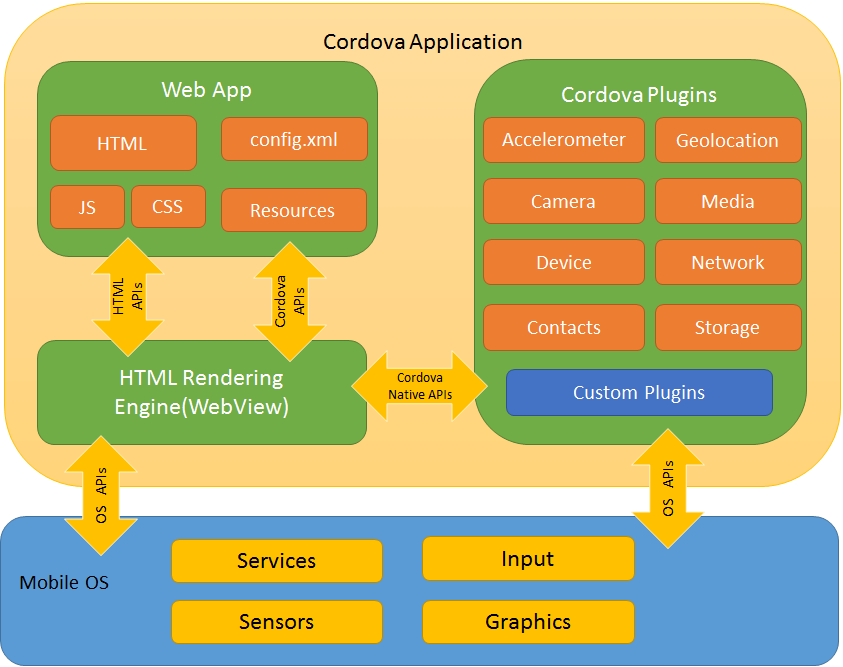
\includegraphics[width=0.6\textwidth]{data/bilder/cordovaapparchitecture.png}
	\caption{Struktureller Aufbau einer Cordova Applikation \cite{cordovaApplicationArchitecture}}
	% https://cordova.apache.org/docs/en/latest/guide/overview/index.html 
	\label{fig:Cordovaapparchitecture}
\end{figure}
%
% --------------------------------------------------------------------------------------------
%
\section{TypeScript}
%
Die von allen modernen Webbrowsern unterstützte Version von JavaScript ist ES5 (ECMAScript 5).
Eine neuere Version von JavaScript, ES6 (ECMAScript 2015), ist eine Obermenge von ES5 was dazu führt, dass ES5-Code stets auch von ES6 unterstützt wird. ES6 wird nicht in vollem Umfang von allen heutigen Browsern unterstützt \cite{compatTableES6}.

TypeScript ist eine von Microsoft entwickelte typisierte Version von ES6, deren Verwendung sich für Ionic 2-Projekte anbietet, da Ionic 2 selbst auch in TypeScript geschrieben ist und so voll typisiert ist \cite{ionic2Docu}.
%https://ionicframework.com/docs/v2/resources/TypeScript/

TypeScript erweitert die Funktioinalitäten von ECMAScript~6 unter anderem um das Konzept fester Datentypen und ermöglicht die Definition eigener Datentypen. Datentypen werden dabei zur Compilezeit überprüft.

Wie aus anderen objektorientierten Programmiersprachen bekannt, verfügen Klassen über das Konzept der Vererbung. Neben Klassen können zudem auch Interfaces definiert werden. Klassen, Interfaces, Funktionen und Variablen können in Modulen in eigenen Namensräumen (\emph{Namespaces}) zusammengefasst werden \cite{MicrosoftTypeScriptDoku}.

Das Konzept der Typisierung von Variablen, den Parametern und Rückgabewerten von Funktionen und die Definition von Interfaces in TypeScript ist in Listing \ref{lst:TypeScriptExample} an einem minimalen Beispiel gezeigt.

\begin{listing}[htb]
    \lstinputlisting{data/sourcecode/typesciptExample.ts}
    \caption{Beispiel zur festen Typisierung in TypeScript}
    \label{lst:TypeScriptExample}
\end{listing}

Wird ein Ionic-Projekt über das Ionic CLI (\enquote{Comand Line Interface}) kompiliert, so findet der sogenannte Transpiling-Vorgang in die vom Browser unterstützte ES5 Version statt. Unter Transpiling, auch source-to-source compiling genannt, wird die Umwandlung von Sourcecode zwischen zwei Programmiersprachen verstanden, die einen ähnlichen Abstraktionslevel besitzen, wohingegen Kompilieren allgemein die Übersetzung von einer Programmiersprache (meist einer high-Level Sprache) in eine andere Sprache (meist eine low-Level Sprache) meint. Transpiling ist also eine spezielle Form des Kompilierens \cite{TranspilingVsCompiling}.
%
% --------------------------------------------------------------------------------------------
%
\section{Angular}
\label{sec:Angular}
%
Angular ist ein von Google entwickeltes clientseitiges JavaScript-Framework zur Erstellung von Single-Page-Webanwendungen. Es arbeitet dabei nach dem Model-View-ViewModel-Entwurfsmuster. Angular baut dabei auf der Erweiterung des Vokabulars von HTML auf und ermöglicht es, Inhalte in der View ohne eine Manipulation des DOM (Document Object Model) anzupassen, ohne selbst JQuery-Manipulationen durchführen zu müssen. Dies geschieht unter Angular mittels Directives.

Die hier betrachtete Version von Angular ist die völlig neugeschriebene Version 2, die auf die Entwicklung mobiler Applikationen ausgelegt ist. Angular 2 ist für die Entwicklung mit der Programmiersprache TypeScript konzipiert. Die finale Version von Angular 2 wurde im September 2016 veröffentlicht.
%
\subsection{Basiskonzepte von Angular 2}
% \cite{DodsonGuideToWebComponents}
% https://css-tricks.com/modular-future-web-components/
Angular 2-Projekte sind in Modulen aufgebaut, die je nach Bedarf mithilfe von imports in andere TypeScript-Dokumente geladen werden können. Als Basiselement werden sogenannte Components verwendet. Components sind wiederverwendbare Komponenten, die einen Teil einer View repräsentieren und dazugehörige Controllerlogik in Form einer TypeScript-Klasse besitzen.

Vor der eigentlichen Klassendefinition werden Components mittels eines decorators eingeleitet, der der Component zusätzliche Informationen wie das zugeordnete Template, das CSS-Style oder den Selector, über den die Component in HTML angesprochen werden kann, liefert. Dieser Mechanismus des Decorators ist in minimaler Form in Listing \ref{lst:decoratorExample} gezeigt.

\begin{listing}[htb]
    \lstinputlisting{data/sourcecode/componentDecoratorExample.ts}
    \caption{Beispiel für einen Decorator einer einfachen Component}
    \label{lst:decoratorExample}
\end{listing}

Innerhalb der TypeScript-Klasse werden Membervariablen und -funktionen bereitgestellt, die aus der View heraus aufgerufen werden können.

HTML5-Templates bilden die View zu einer Component. Mittels Data Binding können die Member der Components mit der View verknüpft werden \cite{LynchAngularComponents}. Data Binding stellt die Datensynchronisation zwischen Model und View dar. Es gibt dabei zwei Arten von Data Binding. One-Way-Data Binding stellt Daten aus dem Model in der View dar. Dies lässt sich in Angular innerhalb der View mittels doppelt geschweiften Klammern realisieren. So werden die im Controller hinterlegten Variablen und Funktionen einseitig mit der View verknüpft. Durch Two-Way-Data Binding mittels der \texttt{ngModel}-Directive lässt sich eine zweiseitige Verknüpfung von View und Model erreichen. Wird die verknüpfte Variable in der View geändert, so wird sie auch im Model angepasst und umgekehrt.

Durch Event Binding werden Elemente einer View mit Angular-Events (z.B. \texttt{focus}, \texttt{blur} und \texttt{click}) oder selbst definierten Events verbunden, die dann Methoden in der jeweiligen Component aufrufen können (vgl. auch  \cite{PrechtAngularTemplateSyntax}).

Angular hat drei Arten von sogenannten Directives: die bereits erwähnten Components, structural Directives und attribute Directives. Directives sind Marker auf einem DOM-Element (z.B. Attribut, Elementname oder CSS-Klasse), die dem Angular HTML-Compiler mitteilen, dass ein bestimmtes Verhalten mit dem jeweiligen DOM-Element verbunden werden soll. Eine Component ist dabei nur eine Spezialform einer Directive mit einem zugeordneten Template.

Mithilfe von \emph{structural Directives} können direkte DOM-Manipulationen vorgenommen werden. So gibt es Angularspezifische Directives wie beispielsweise die  \texttt{*ngFor}-Directive, die wie eine foreach-Schleife einen Container durchlaufen kann und so z.B. schnell eine Tabelle erstellen kann. Ähnlich bedeutend ist die \texttt{*ngIf}-Directive mit deren Hilfe selektiv an eine Bedingung geknüpft Elemente erzeugt werden können.

\emph{Attribute Directives} ändern das Verhalten oder Aussehen bestehender Elemente. So kann beispielsweise mittels der \texttt{ngModel}-Directive ein Two-Way-Data Binding mit einem Attribut einer Component realisiert werden. 

Mittels Referenzen auf einzelne Element des DOM können aus einem Element direkt andere Elemente innerhalb der View angesprochen werden.

Services sind Klassen, die wiederverwendbare Funktionalitäten für Components bereitstellen. Grundsätzlich sollten Components so schlank wie möglich konzipiert sein und die eigentliche Funktionalität sollte in Services ausgelagert werden, um eine wiederverwendbarkeit von Funktionalitäten zu ermöglichen und die Programmlogik übersichtlich zu halten. So sollten Components selbst keine Serveranfragen durchführen oder Daten validieren. Stattdessen sollten solche Aufgaben an Services weitergeleitet werden, die dann in verschiedenen Components Verwendung finden können.
%
Mithilfe des \emph{Dependency injection} Entwurfsmusters \cite{angularDependencyInjectionDoku} werden Components zur Laufzeit mit neuen Instanzen der Services versorgt, die sie benötigen. So werden stets nur die Service-Klassen geladen, die wirklich benötigt werden \cite{angularDocuBasicArchitecture}. Dependency injection findet in Angular 2 über den Konstruktor der Component-Klasse statt. Hier werden die benötigten Abhängigkeiten der Component als Argumente mit übergeben.
%
% --------------------------------------------------------------------------------------------
%
\section{Konzepte des Ionic 2 Frameworks mit Angular 2}
\label{sec:ionicKonzepte}

Das Ionic-Framework liefert eine große Sammlung an Angular 2-Components die sich frei in ein Cordova-Projekt einbauen lassen. Es liefert zudem verschiedene Styles pro Plattform, die durch komplett verschiedene und unabhängige SASS-Dateien realisiert werden. So sorgt Ionic 2 für ein plattformspezifisches Nutzererlebnis. Eine große über 900 Elemente umfassende Sammlung an Icons, die sogenannten Ionicons, passt sich zudem dynamisch dem jeweiligen Betriebssystem an und liefert so ebenfalls einen möglichst passenden Stil, der zur jeweiligen Plattform passt. Ionic Native ist eine Sammlung an TypeScript-Wrappern für Cordova- bzw. PhoneGap-Plugins, also an das Ionic Framework und die Nutzung von Angular zur Erstellung der Webapp angepasste und typisierte Cordova-Plugins, die es ermöglichen grundsätzlich jede Art von nativer Funktionalität zu einer Ionic-App hinzuzufügen \cite{ionic2Docu}.
% https://ionicframework.com/docs/v2/native/

Der große Vorteil in der Verwendung des Ionic-Frameworks ist, dass bereits eine große Zahl an Components vorgefertigt sind, die ansonsten zunächst selbst erstellt und im Style an die jeweilige Plattform einzeln angepasst werden müssten. So liefert Ionic bereits viele für mobile Plattformen typische vorgefertigte Steuerelemente wie Buttons, Listen, Eingabefelder, Checkboxen oder ähnlichen für mobile Geräte typischen Komponenten, die zudem ein den nativen Elementen nachempfundenes Verhalten sowie Styling besitzen. All diese Funktionalitäten lassen sich auch ohne das Ionic Framework realisieren, jedoch wäre dies mit einem sehr großen Mehraufwand verbunden. 

Listing \ref{lst:ionicExampleView} zeigt exemplarisch eine typische View-Implementierung einer Liste (Table-View) mittels der \texttt{ion-list}-, \texttt{ion-item}- und \texttt{ion-thumbnail}-Components. Die Component \texttt{ion-list} erstellt dabei eine Table-View, \texttt{ion-item} liefert eine einzelne Tabellenzeile und \texttt{ion-thumbnail} bietet die Möglichkeit ein kleines Bild in eine Table-View-Zeile einzubinden.

\begin{listing}[htb]
    \lstinputlisting{data/sourcecode/ionicExample.html}
    \caption{Beispiel einer typischen \texttt{ion-list}}
    \label{lst:ionicExampleView}
\end{listing}

Dabei werden mittels der Angular Direktive \texttt{*ngFor} Elemente eines Arrays (hier \enquote{talkers}) aufgelistet. Mittels der in doppelten geschweiften Klammern geschriebenen One-Way-Data Bindings kann auf die Attribute des betrachteten Objektes (hier \enquote{\#talker}) der Schleife zugegriffen werden. Die einzelnen \texttt{ion-item}s werden zudem mit einem Click-Event verknüpft, welches hier eine in der Component implementierten Methode \enquote{\texttt{goToDetailView}} aufruft. Die \texttt{*ngIf}-Bedingung sorgt dafür, dass nur bei erfüllter Bedingung das \texttt{<span>}-Element erzeugt wird.

Listing \ref{lst:ionicExampleTs} zeigt die minimal gehaltene TypeScript-Component zur in Listing \ref{lst:ionicExampleView} dargestellten HTML-View. Ein Interface \texttt{ITalker} definiert den in der View dargestellten Datentyp. Mittels dependency-injection wird ein externer Service namens \texttt{DatabaseService} eingebunden, der im Konstruktor über die Methode des Services \texttt{getTalkersArray} die darzustellenden das Interface \texttt{ITalker} implementierende Objekte in einem Array liefert. Die in der Component definierte Funktion \texttt{goToDetailView}, welche als Parameter ein Objekt vom zuvor definierten Interfacetyp \texttt{ITalker} erwartet, kann über die View aufgerufen werden.

\begin{listing}[htb]
    \lstinputlisting{data/sourcecode/ionicExample.ts}
    \caption{Beispiel einer einfachen Component-Implementation}
    \label{lst:ionicExampleTs}
\end{listing}

Die hier verwendeten Components \texttt{ion-list}, \texttt{ion-item} sowie \texttt{ion-thumbnail} bilden einen sehr komfortablen Weg, auf einfache Art und Weise für mobile Plattformen angepasste Listen zu erstellen. Würde hier auf die Verwendung des Ionic-Frameworks verzichtet müssten diese Components zunächst selbst entwickelt werden.
%
%
% --------------------------------------------------------------------------------------------
% ================================
% = Nicht im Dokument enthalten! =
% ================================
\begin{comment}

\section{Struktur eines Ionic 2-Projektes} 
% https://ionicframework.com/docs/v2/getting-started/tutorial/project-structure/
% http://codingthesmartway.com/ionic-2-project-structure/
\subsection*{./src/}
%
\todo{Soll das Kapitel "Struktur eines Ionic 2-Projektes" raus?}
%
Innerhalb des src-Ordners liegt der unkompillierte TypeScriptcode sowie die Templates. Wird der Buildvorgang per CLI in Gang gesetzt, wird der Code im src-Ordner mittels Transpiling in die korrekte JavaScriptversion umgewandelt und in den www-Ordner kopiert.

Im Unterordner \texttt{./src/app/} wird die Haupt-Komponente der App gespeichert. Diese bildet den Eintrittspunkt der App, das sogenannte \emph{root module} aus dem heraus alle anderen Komponenten geladen werden.

Im Unterordner \texttt{./src/pages/} werden alle weiteren Unterseiten der App mit ihren Komponenten gespeichert. Jede Page besteht dabei aus einem weiteren Unterordner mit grundsätzlich je einer View (.html), einer Komponente (.ts) und der zugehörigen Style-Datei (.scss).
%
\subsection*{./src/index.html}
In der \texttt{index.html} werden benötigte Scripte und Styles geladen und die eigentliche ionic-App wird mit dem \texttt{<ion-app>}-Tag gestartet. Zudem werden die benötigten Skripte \texttt{cordova.js} und \texttt{build/main.js} geladen.
%
\subsection*{./resources/}
Im Ordner \texttt{resources} liegen die für die App nötigen je nach Plattform typischen Icons und Splashscreens (Startbildschirmbilder). 
%
\subsection*{./assets/}
Im Ordner \texttt{assets} werden Ressourcen der App bereitgestellt, die bereits zu Beginn zur Verfügung gestellt werden sollen. So können Datenbanken bereitgestellt werden oder Bilder abgelegt werden.
%
\end{comment}